% Figure 1 of the MDPI version, compiled once into figures/cascade_diagram.pdf (see README.md) so that the
% article itself needs no TikZ libraries. Same fonts as the article: T1 + mathpazo (Palatino), 10 pt base size.
\documentclass[border=2pt]{standalone}
\usepackage[T1]{fontenc}
\usepackage{mathpazo}
\usepackage{tikz}
\usetikzlibrary{arrows.meta,positioning,shapes.geometric}
\begin{document}
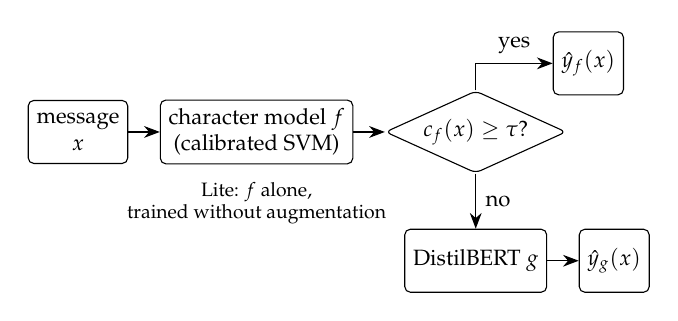
\begin{tikzpicture}[font=\footnotesize, node distance=4mm,
  box/.style={draw, rounded corners=2pt, align=center, minimum height=8mm, inner sep=3pt},
  arr/.style={-{Stealth[length=2mm]}}]
\node[box] (x) {message\\$x$};
\node[box, right=of x] (f) {character model $f$\\(calibrated SVM)};
\node[below=1mm of f, font=\scriptsize, align=center] {Lite: $f$ alone,\\trained without augmentation};
\node[box, diamond, aspect=2.2, inner sep=1pt, right=of f] (d) {$c_f(x)\ge\tau$?};
\node[box, above right=2mm and 4mm of d] (y1) {$\hat{y}_f(x)$};
\node[box, below=7mm of d] (g) {DistilBERT $g$};
\node[box, right=4mm of g] (y2) {$\hat{y}_g(x)$};
\draw[arr] (x) -- (f);
\draw[arr] (f) -- (d);
\draw[arr] (d) |- node[pos=0.75, above] {yes} (y1);
\draw[arr] (d) -- node[right] {no} (g);
\draw[arr] (g) -- (y2);
\end{tikzpicture}
\end{document}
